\documentclass[
11pt, % The default document font size, options: 10pt, 11pt, 12pt
%codirector, % Uncomment to add a codirector to the title page
]{charter} 
% El títulos de la memoria, se usa en la carátula y se puede usar el cualquier lugar del documento con el comando \ttitle
\titulo{Desarrollo de aplicación Hospitalaria con MQTT} 

% Nombre del posgrado, se usa en la carátula y se puede usar el cualquier lugar del documento con el comando \degreename
%\posgrado{Carrera de Especialización en Sistemas Embebidos} 
\posgrado{Carrera de Especialización en Internet de las Cosas} 
%\posgrado{Carrera de Especialización en Intelegencia Artificial}
%\posgrado{Maestría en Sistemas Embebidos} 
%\posgrado{Maestría en Internet de las cosas}

% Tu nombre, se puede usar el cualquier lugar del documento con el comando \authorname
\autor{Ing. Gustavo Bastian} 

% El nombre del director y co-director, se puede usar el cualquier lugar del documento con el comando \supname y \cosupname y \pertesupname y \pertecosupname
\director{Mg.Ing. Ericson Joseph Estupiñan Pineda}
\pertenenciaDirector{Surix S.R.L} 
% FIXME:NO IMPLEMENTADO EL CODIRECTOR ni su pertenencia
%\codirector{John Doe} % para que aparezca en la portada se debe descomentar la opción codirector en el documentclass
%\pertenenciaCoDirector{FIUBA}

% Nombre del cliente, quien va a aprobar los resultados del proyecto, se puede usar con el comando \clientename y \empclientename
\cliente{Ing. Sergio Starkloff}
\empresaCliente{Surix S.R.L}

% Nombre y pertenencia de los jurados, se pueden usar el cualquier lugar del documento con el comando \jurunoname, \jurdosname y \jurtresname y \perteunoname, \pertedosname y \pertetresname.
\juradoUno{Nombre y Apellido (1)}
\pertenenciaJurUno{pertenencia (1)} 
\juradoDos{Nombre y Apellido (2)}
\pertenenciaJurDos{pertenencia (2)}
\juradoTres{Nombre y Apellido (3)}
\pertenenciaJurTres{pertenencia (3)}
 
\fechaINICIO{31 de Octubre de 2021}		%Fecha de inicio de la cursada de GdP \fechaInicioName
\fechaFINALPlan{7 de Diciembre de 2021} 	%Fecha de final de cursada de GdP
\fechaFINALTrabajo{15 de mayo de 2022}	%Fecha de defensa pública del trabajo final


\begin{document}

\maketitle
\thispagestyle{empty}
\pagebreak


\thispagestyle{empty}
{\setlength{\parskip}{0pt}
\tableofcontents{}
}
\pagebreak


\section*{Registros de cambios}
\label{sec:registro}


\begin{table}[ht]
\label{tab:registro}
\centering
\begin{tabularx}{\linewidth}{@{}|c|X|c|@{}}
\hline
\rowcolor[HTML]{C0C0C0} 
Revisión & \multicolumn{1}{c|}{\cellcolor[HTML]{C0C0C0}Detalles de los cambios realizados} & Fecha      \\ \hline
0      & Creación del documento                                 & 31/10/2021 \\ \hline
1      & Se completa hasta el punto 5 inclusive                 & 3/11/2021 \\ \hline
2      & Se completa hasta el punto 9 inclusive
& 11/11/2021 \\ \hline
3      & Se corrigen historias de usuario y se completa hasta el punto 12 inclusive
& 18/11/2021 \\ \hline
4      & Se completa la totalidad del documento
& 25/11/2021 \\ \hline
5      & Se corrige el punto 14 y la ubicación de graficos de diagramas de AoN.
& 7/12/2021 \\ \hline
%		  Se puede agregar algo más \newline
%		  En distintas líneas \newline
%		  Así                                                    & dd/mm/aaaa \\ \hline
%3      & Se completa hasta el punto 11 inclusive                & dd/mm/aaaa \\ \hline
%4      & Se completa el plan	                                 & dd/mm/aaaa \\ \hline
\end{tabularx}
\end{table}

\pagebreak



\section*{Acta de constitución del proyecto}
\label{sec:acta}

\begin{flushright}
Buenos Aires, \fechaInicioName
\end{flushright}

\vspace{2cm}

Por medio de la presente se acuerda con el Ing. \authorname\hspace{1px} que su Trabajo Final de la \degreename\hspace{1px} se titulará ``\ttitle''. Consistirá esencialmente en {la implementación de un prototipo de una aplicación móvil para la llamada, gestión de enfermeras y consulta enfermera-médico mediante la utilización del protocolo MQTT}, y tendrá un presupuesto preliminar estimado de {620} hs de trabajo y {\$649400}, con fecha de inicio \fechaInicioName\hspace{1px} y fecha de presentación pública \fechaFinalName.

Se adjunta a esta acta la planificación inicial.

\vfill

% Esta parte se construye sola con la información que hayan cargado en el preámbulo del documento y no debe modificarla
\begin{table}[ht]
\centering
\begin{tabular}{ccc}
\begin{tabular}[c]{@{}c@{}}Dr. Ariel Lutenberg \\ Director posgrado FIUBA\end{tabular} & \hspace{2cm} & \begin{tabular}[c]{@{}c@{}}\clientename \\ \empclientename \end{tabular} \vspace{2.5cm} \\ 
\multicolumn{3}{c}{\begin{tabular}[c]{@{}c@{}} \supname \\ Director del Trabajo Final\end{tabular}} \vspace{2.5cm} \\
%\begin{tabular}[c]{@{}c@{}}\jurunoname \\ Jurado del Trabajo Final\end{tabular}     &  & \begin{tabular}[c]{@{}c@{}}\jurdosname\\ Jurado del Trabajo Final\end{tabular}  \vspace{2.5cm}  \\
%\multicolumn{3}{c}{\begin{tabular}[c]{@{}c@{}} \jurtresname\\ Jurado del Trabajo Final\end{tabular}} \vspace{.5cm}                                                                     
\end{tabular}
\end{table}




\section{1. Descripción técnica-conceptual del proyecto a realizar}
\label{sec:descripcion}


En la actualidad, el avance de la Internet de las Cosas (IoT de \textit{Internet of Things}) y la disminución de costos asociados a la tecnología hacen factible su incorporación a distintos campos de la vida cotidiana. Uno de esos campos es el de infraestructuras hospitalarias inteligentes. 

Por otra parte, dentro de las múltiples opciones para realizar la comunicación entre los dispositivos IoT, el protocolo Message Queuing Telemetry Transport (en adelante MQTT) se ha probado como un protocolo confiable y ampliamente utilizado.

Dentro del contexto, en este trabajo se desarrollará una aplicación multiplataforma que utilizará el protocolo MQTT para los distintos participantes  de la actividad hospitalaria. El proyecto es una necesidad de la empresa Surix S.R.L. y se lleva a cabo como parte de la carrera Especialización de Internet de las Cosas.

Surix S.R.L. es una firma que se dedica al desarrollo, fabricación y comercialización de productos IP y sistemas hospitalarios de calidad. Posee una comprobada trayectoria dentro del mercado local e internacional. Se destaca por su compromiso con la industria nacional, la mejora continua de sus productos y el soporte que brinda a sus clientes. Este proyecto se enmarca dentro del segundo ítem de su misión, porque mejora y extiende capacidades a un sistema existente. 

Surix S.R.L fabrica un sistema IP de llamado a enfermera que está basado en el protocolo SIP. Este consiste en un servidor central y terminales que se encuentran en las habitaciones del hospital. La aplicación principal se ejecuta en una pc o bien en una tablet y monitorea el estado de las habitaciones. 
 
El objetivo del proyecto es realizar un sistema con las ventajas que provee el protocolo MQTT, como es la posibilidad de agregar accesorios rápidamente con bajo costo de software, hardware e implementación. 

MQTT es un protocolo open source liviano, hecho que permite aplicarlo en dispositivos con pocos recursos y baja velocidad de transmisión, ampliamente utilizado en dispositivos IoT. Está basado en la pila TCP/IP, se implementa en la capa de aplicación y sus mensajes se transmiten como colas de publicación/subscripción. 

El desafío de este proyecto consiste en la programación de un sistema que contenga un servidor o broker MQTT, una base de datos donde alojar información de reportes de habitaciones/enfermeras y datos relevantes al paciente (incluyendo temporizadores para suministro de ciertos medicamentos y/o control), una página web para configuración y una aplicación multiplataforma donde se realice la gestión de datos e interacción con los clientes. La aplicación será capaz de identificar la cama correspondiente (mediante lectura de símbolos QR) y de transmitir mensajes de voz en caso de ser necesario.

La motivación que origina la realización del proyecto es generar las bases para poder incorporar otros dispositivos inteligentes al sistema principal a bajo costo. Por ejemplo, en un futuro se puede monitorear la temperatura de la habitación y saber si sufre un desperfecto el aire acondicionado, escuchar sonidos dentro de la sala en caso de que el paciente no pueda acceder al llamador, etc.

%El objetivo es que el lector en una o dos páginas entienda de qué se trata el 
%proyecto y cuáles son sus desafíos, su motivación y su importancia.

%Se debe destacar claramente cuál es el valor que agrega el proyecto a realizar. 
%``El presente proyecto se destaca especialmente por incorporar tal cosa... Esto 
%lo diferencia de otros sistemas similares en que ...''

%Puede ser útil incluir en esta sección la respuesta a alguna de estas preguntas:

%\begin{itemize}
%	\item ¿Cómo se vincula este proyecto con la misión de la %organización?
%	\item ¿Cómo se inserta este proyecto en el modelo de negocio de la organización?
%	\item ¿Ayuda a la explicación si se incluye un lienzo Canvas del Modelo de Negocio?
%	\item ¿En qué estado del ciclo de vida está el producto que se desea reemplazar o mejorar?
%	\item ¿Cuáles son las necesidades que debe satisfacer?
%	\item ¿Por dónde pasa la innovación?
%\end{itemize}
%
%La descripción técnica-conceptual \textbf{debe incluir al menos un diagrama en bloques del sistema} y una frase como la siguiente: ``En la Figura \ref{fig:diagBloques} se presenta el diagrama en bloques del sistema. Se observa que...''. Luego recién más abajo de haber puesto esta frase, se pone la figura. La regla es que las figuras nunca pueden ir antes de ser mencionadas en el texto, porque sino el lector no entiende por qué de pronto aparece una figura.

\vspace{50px}

El proyecto completo consta de :
\begin{itemize}
\item Broker.
\item Pantalla web de configuración.
\item Cliente médico.
\item Cliente enfermera.
\item Cliente sistema.
\end{itemize}
En la figura 1 se presenta un diagrama de interconexión entre los dispositivos.


%\vspace{25px}

\begin{figure}[htpb]
\centering 
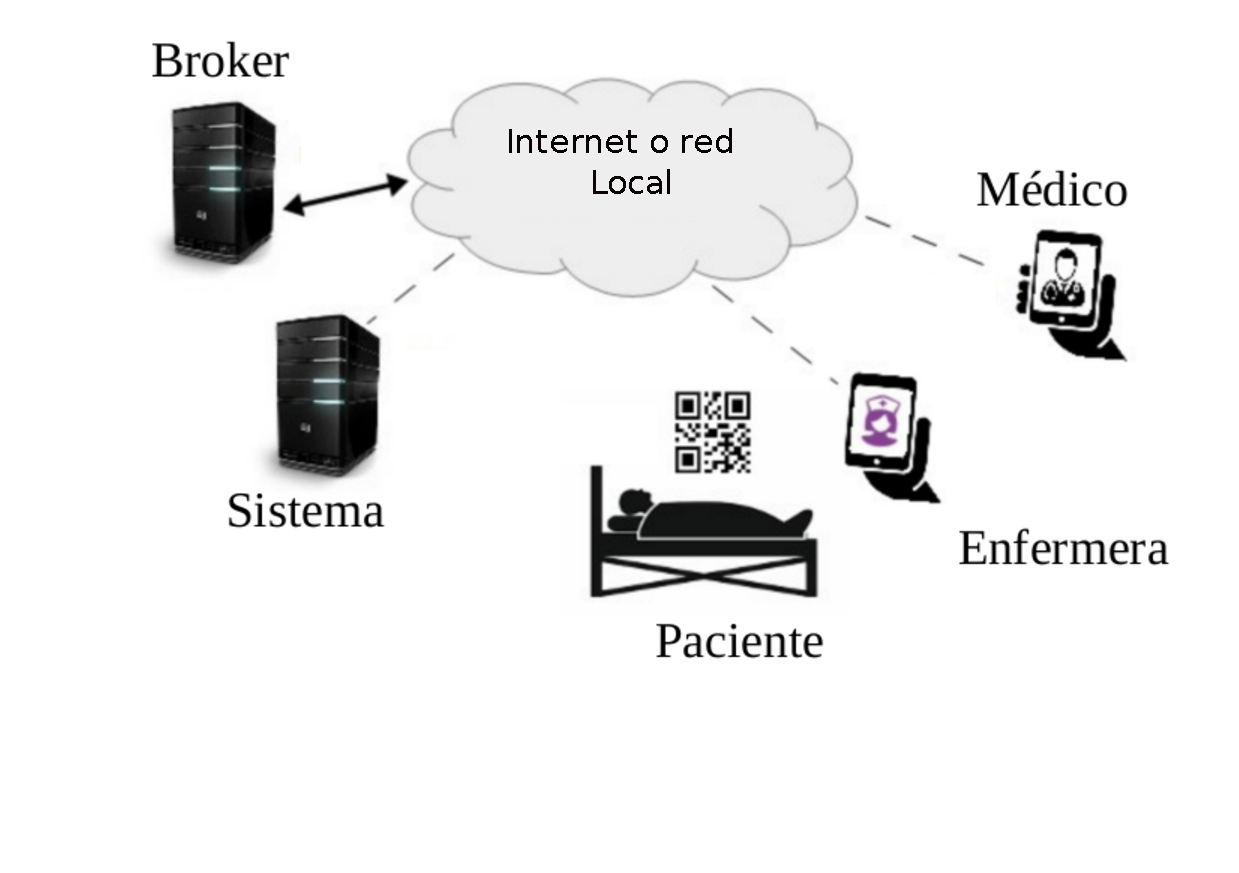
\includegraphics[width=.7\textwidth]{./Figuras/diag3.pdf}
\caption{ Diagrama en bloques del sistema.}
\label{fig:diagBloques}
\end{figure}

%\vspace{25px}

El broker recibe mensajes llamados ``eventos'', de distintos publicadores y los reenvía a los subscriptores que correspondan según una política asignada previamente. El cliente sistema puede gestionar la base de datos con información relevante para los pacientes y también puede observar el estado de las habitaciones. Mientras que el cliente enfermera solo recibe asignaciones o respuestas de un médico, y publica finalización o consulta por medio de la aplicación. Por último, el cliente médico solo recibe consultas y publica respuestas por medio de la aplicación.

Con la aplicación web se puede cargar la base de datos con información de enfermeras, pacientes y médicos.
\vfill

 
%El tamaño de la tipografía en TODAS las figuras debe ser adecuado para que NO pase lo que ocurre acá, donde el lector debe esforzarse para poder leer el texto. Los colores usados en el diagrama deben ser adecuados, tal que ayuden a comprender mejor el diagrama, preferentemente en la gama de colores pastel.



\section{2. Identificación y análisis de los interesados}
\label{sec:interesados}


%Nota: (borrar esto y todas las consignas en color rojo antes de entregar este documento).
 
%Es inusual que una misma persona esté en más de un rol, incluso en proyectos chicos.
 
%Si se considera que una persona cumple dos o más roles, entonces sólo dejarla en el rol más importante. Por ejemplo:

%Pero en cambio sí es usual que el Cliente y el Auspiciante sean el mismo, por ejemplo.

\begin{table}[H]
%\caption{Identificación de los interesados}
%\label{tab:interesados}
\begin{tabularx}{\linewidth}{@{}|l|X|X|l|@{}}
\hline
\rowcolor[HTML]{C0C0C0} 
Rol           & Nombre y Apellido & Organización 	& Puesto 	\\ \hline
%Auspiciante   &                   &              	&        	\\ \hline
Cliente       & \clientename      &\empclientename	& Propietario       	\\ \hline
%Impulsor      &                   &              	&        	\\ \hline
Responsable   & \authorname       & FIUBA        	& Alumno 	\\ \hline
Colaboradores & --                   & --             	& --       	\\ \hline
Orientador    & \supname	      & \pertesupname 	& Director trabajo final \\ \hline
%Equipo        & miembro1 \newline 
%				miembro2          &              	&        	\\ \hline
%Opositores    &                   &              	&        	\\ \hline
Usuario final &personal de salud, administradores de sistemas         &  --            	&  --      	\\ \hline
\end{tabularx}
\end{table}

%El Director suele ser uno de los Orientadores.

%No dejar celdas vacías; si no hay nada que poner en una celda colocar un signo ``-''.

%No dejar filas vacías; si no hay nada que poner en una fila entonces eliminarla.

%Es deseable listar a continuación las principales características de cada interesado.
 
%Por ejemplo:
\begin{itemize}
%	\item Auspiciante: es riguroso y exigente con la rendición de gastos. Tener mucho cuidado con esto.
%	\item Equipo: Juan Perez, suele pedir licencia porque tiene un familiar con una enfermedad. Planificar considerando esto.
%	\item Orientador: María Gómez va a poder ayudar mucho con la definición de los requerimientos.
\item Orientador: Ericson va a poder ayudar mucho con la definición de los requerimientos.
\item Usuario final: Todos los usuarios del sistema como ser, administradores de redes hospitalarias, médicos y enfermeras, que deseen observar y/o controlar el proceso.

\end{itemize}





\section{3. Propósito del proyecto}
\label{sec:proposito}



El propósito de este proyecto es desarrollar un sistema para gestión de enfermeras basado en el protocolo MQTT compuesto por un broker, una web de configuración y una o varias aplicaciones, que agilice el desarrollo de funcionalidades futuras.
%¿Por qué se hace el proyecto? ¿Qué se quiere lograr? 

%Se recomienda que sea solo un párrafo que empiece diciendo ``El propósito de este proyecto es...''.


\section{4. Alcance del proyecto}
\label{sec:alcance}

%¿Qué se incluye y que no se incluye en este proyecto?

%Se refiere al trabajo a hacer para entregar el producto o resultado especificado. 

%Explicitar todo lo quede comprendido dentro del alcance del proyecto.

%Explicitar además todo lo que no quede incluido (``El presente proyecto no incluye...'')
El presente proyecto incluye:

\begin{itemize}
	\item Confección del plan de trabajo. 
	\item Investigación y estudio del protocolo MQTT, bases de datos SQL y NoSQL, programación de aplicaciones web y programación de aplicaciones multiplataforma.	
	\item Desarrollo local del broker que registre en un log las actividades realizadas y su horario de realización. 
	\item Desarrollo local de una página web de configuración.
	\item Desarrollo local de una aplicación con 3 modos de funcionamiento : modo médico con envío/recepción de mensajes de audio/texto/alarmas; modo enfermera con envío/recepción de mensajes de audio/texto/alarmas y escaneo de QR para identificar paciente; y modo sistema que asigna enfermeras a pacientes de acuerdo a la indicación de un médico. Por ejemplo, todos los días a las 17 hs, medir la presión arterial del paciente ``x", independientemente de la enfermera. Esta aplicación en modo sistema permite monitorizar el estado de las habitaciones.
	\item Documentación de las aplicaciones desarrolladas.

\end{itemize}

El presente proyecto NO incluye:
\begin{itemize}
	\item Manuales de las distintas aplicaciones desarrolladas.
	\item Traducciones a idiomas extranjeros de las aplicaciones y/o de la página web.
	\item Sistema llamador del paciente.
	\item Análisis en profundidad de tráfico en la red.
	\item Análisis en profundidad de Seguridad.
	\item Contratación de base de datos remota.
	\item Contratación e instalación de servidores remotos.
\end{itemize}



\section{5. Supuestos del proyecto}
\label{sec:supuestos}
Para el desarrollo del presente proyecto se supone que: 

\begin{itemize}
	\item Existe un llamador paciente. 
	\item Las aplicaciones moviles usaran iOS y Android como sistema operativo.
	\item La base de datos de los pacientes sólo puede ser afectada por medio de la aplicación sistema (el cliente médico sólo puede hacer consultas/modificaciones puntuales a una situación).	
	\item Se dispondrá al menos de una pc para instalación del servidor web, la base de datos, y del broker MQTT.
	\item Se dispondrá de un router para la prueba funcional del sistema. 

\end{itemize}

%\begin{consigna}{red}
%``Para el desarrollo del presente proyecto se supone que: ...''

%\begin{itemize}
%	\item Supuesto 1
%	\item Supuesto 2...
%\end{itemize}

%Por ejemplo, se podrían incluir supuestos respecto a disponibilidad de tiempo y recursos humanos y materiales, sobre la factibilidad técnica de distintos aspectos del proyecto, sobre otras cuestiones que sean necesarias para el éxito del proyecto como condiciones macroeconómicas o reglamentarias.
%\end{consigna}



\section{6. Requerimientos}
\label{sec:requerimientos}
Los principales requerimientos relevados son los siguientes:

\begin{enumerate}
	\item Requerimientos funcionales del servidor:
			\begin{enumerate}
			\item El servidor debe tener instalado Eclipse Mosquitto como broker MQTT.
			\item El servidor debe tener endpoints para interactuar con una aplicación Web, para consultas y envío de datos hacia dispositivos clientes.
			\item El servidor debe tener endpoints para interactuar con la base de datos.

			
			\end{enumerate}
	\item Requerimientos funcionales de la base de datos:
		\begin{enumerate}		
			\item El sistema debe poseer una base de datos relacional.
			\item La base de datos debe poseer datos cargados por default.
			\item La base de datos a utilizar debe poseer las siguientes tablas:
			\begin{itemize}
			
				\item Habitaciones
						
				\item Pacientes			
			
				\item Médicos
			
				\item Enfermeras			
			
				\item Eventos 
			\end{itemize}
		\end{enumerate}	
	\item Requerimientos funcionales de la aplicación web de configuración:
		\begin{enumerate}	
		\item La aplicación web debe ser cliente del broker MQTT.
		\item La aplicación web debe poseer funciones de consulta o modificación de la base de datos.
		\item La aplicación web debe ser permitir visualización de estadísticas de pacientes o enfermeras.
		\item La aplicación debe contener acceso con usuario y contraseña para cada persona.
		\end{enumerate}			
	
	
	
	\item Requerimientos funcionales de la aplicación enfermera:
		\begin{enumerate}
			\item La aplicación enfermera debe tener 3 modos de uso: usuario médico, usuario enfermera y usuario sistema.
			\item Al logearse el usuario, y contrastarse con la base de datos del sistema, se activa el modo correspondiente.
			\item La aplicación en modo enfermera debe permitir leer códigos QR.			
			\item La aplicación en modo enfermera debe poder descargar información relevante del paciente (medicamentos a suministrar, controles a realizar, contacto del médico a cargo del tratamiento, etc).	
			\item La aplicación en modo sistema debe mostrar las habitaciones sin atención, según una tabla de prioridades y en caso de igualdad de prioridades, mostrár según el orden de llamada.
			\item El modo usuario médico y el modo usuario enfermera deben poder enviar mensajes de textos o sonido comprimido en 32kbps (mp3).
		\end{enumerate}
		
		
	\item Requerimientos de documentación:
		\begin{enumerate}
			\item Confección de documento con información relativa a la base de datos: detalles de la misma y de API para acceder.
			\item Memoria del proyecto con diagramas UML de aplicación modo sistema, aplicación modo enfermera, aplicación modo médico y página web.
			
		\end{enumerate}
		
		
	\item Requerimientos de integración de sistema:	
			\begin{enumerate}
			\item El sistema debe integrar el funcionamiento del servidor con base de datos , aplicación web y aplicaciones moviles.			
			\end{enumerate}	
			
	\item Requerimientos de entrega del producto:	
			\begin{enumerate}
			\item El código fuente del servidor debe ser subido a dockerhub y compartido con la comunidad.	
			\item El código fuente de la aplicación debe ser subido a github y compartido con la comunidad.
			\end{enumerate}			
	

\end{enumerate}


\section{7. Historias de usuarios (\textit{Product backlog})}
\label{sec:backlog}

%\begin{consigna}{red}
%Descripción: En esta sección se deben incluir las %historias de usuarios y su ponderación (\textit{history %points}). Recordar que las historias de usuarios son descripciones cortas y simples de una característica contada desde la perspectiva de la persona que desea la nueva capacidad, generalmente un usuario o cliente del sistema. La ponderación es un número entero que representa el tamaño de la historia comparada con otras historias de similar tipo.

%El formato propuesto es: "como [rol] quiero [tal cosa] para [tal otra cosa]."

%Se debe indicar explícitamente el criterio para calcular los \textit{story points} de cada historia
%\end{consigna}
Se identifican los siguientes roles:
\begin{itemize}
	\item Usuario final: persona que utilizará el sistema. Existen  usuarios finales bien definidos: usuario final modo enfermero, usuario final modo médico y usuario final modo operador del sistema.
	\item Cliente: persona que necesita el desarrollo. Sus intereses están orientados al negocio.

\end{itemize}

Story points:
Se utilizarán 1, 2, 3, 5 y 8 para la estimación de las historias de usuario, según la serie de Fibonacci.
\begin{itemize}
	\item Historias de 1 punto: son historias cuya implementación es rápida 	y con baja posibilidad de falla. Por ejemplo envío de un mensaje 			sencillo entre un nodo y el servidor de la red.
	\item Historias de 2 puntos: son historias cuya implementación no es rápida, pero tienen baja posibilidad de falla. Por ejemplo el diseño de la interfaz de usuario.
	\item Historias de 3 puntos: son historias cuya implementación no es rápida y tienen una posibilidad de falla media. Por ejemplo para la lectura de códigos QR es necesario investigar bibliotecas y evaluar el correcto funcionamiento en dispositivos con sistemas operativos distintos.
	\item Historias de 5 puntos: son historias cuya implementación es lenta y poseen una posibilidad de falla alta ya que interactúan varios elementos de la red. Por ejemplo el envío de un mensaje de audio entre distintos actores, debido a que hay que corroborar el funcionamiento de la captura de audio en ambos dispositivos, el correcto traslado por la red y la recepción perfecta del archivo.
	\item Historias de 8 puntos: son historias cuya implementación es compleja y poseen  elevada posibilidad de falla porque interactúan distintos componentes del sistema. Por ejemplo en la solicitud de ayuda de una enfermera al sistema, donde se debe chequear disponibilidad de otras enfermeras, y dependiendo del tipo de ayuda necesaria, la capacidad de la misma.

\end{itemize}

Historias de Usuario:

\begin{itemize}
\item Como usuario en modo enfermero quiero que la aplicación me notifique si hay un pedido de una habitación para ir a atenderla. Dificultad baja y posibilidad de falla  baja. (1 punto)

\item Como usuario en modo enfermero quiero que la aplicación permita que notifique que finalicé la tarea para poder recibir otro pedido. Dificultad baja y posibilidad de falla  baja. (1 punto)

\item Como usuario en modo enfermero quiero que la aplicación me permita notificar que estoy atendiendo para no tener varios pedidos pendiente. Dificultad media y posibilidad de falla media. (3 puntos)

\item Como usuario en modo enfermero quiero que la aplicación permita que consulte a un médico en caso de necesidad. Dificultad muy alta y posibilidad de falla muy alta. (8 puntos)

\item Como usuario en modo enfermero quiero que la aplicación permita obtener información del paciente para entender el estado de la situación. Dificultad alta y posibilidad de falla alta. (5 puntos)

\item Como usuario en modo enfermero quiero que la aplicación permita avisar que mi jornada terminó para no recibir más notificaciones. Dificultad alta y posibilidad de falla alta. (5 puntos)

\item Como usuario en modo enfermero quiero que la aplicación permita que notifique que necesito ayuda de otro enfermero para atender al paciente. Dificultad muy alta y posibilidad de falla muy alta. (8 puntos)

\item Como usuario en modo médico quiero que la aplicación posea un mecanismo sencillo para responder dudas de la enfermera. Dificultad media y posibilidad de falla media. (3 puntos)

\item Como usuario en modo médico quiero que la aplicación permita acceder a la información del paciente en caso de consulta de un enfermero. Dificultad media y posibilidad de falla baja. (2 puntos)

\item Como usuario en modo sistema quiero que la aplicación me permita asignar tareas temporizadas para atender rutinas preestablecidas por el médico. Dificultad alta y posibilidad de falla alta. (5 puntos)

\item Como usuario en modo sistema quiero que la aplicación permita obtener datos estadísticos de cada enfermero para poder reportar. Dificultad media y posibilidad de falla baja. (2 puntos)

\item Como usuario en modo sistema quiero que la aplicación móvil me muestre el estado de las habitaciones. Dificultad baja y posibilidad de falla baja. (1 punto)

\item Como cliente quiero que el sistema sea de fácil instalación. Dificultad baja y posibilidad de falla baja. (1 punto)

\end{itemize}

\section{8. Entregables principales del proyecto}
\label{sec:entregables}



Los entregables del proyecto son:

\begin{itemize}
	\item Plan de proyecto del trabajo final y memoria técnica.
	\item Servidor MQTT.
	\item Base de datos configurada.
	\item Aplicación Web responsive.
	\item Aplicación enfermera (con los 3 modos de funcionamiento).
	\item Código del sistema (utilizando dockerhub y github).
\end{itemize}

\section{9. Desglose del trabajo en tareas}
\label{sec:wbs}

Desglose del trabajo:

\begin{enumerate}
\item Investigación preliminar (70 hs):
	\begin{enumerate}
	\item Confección del plan de trabajo del proyecto (10 hs).
	\item Investigar funcionamiento del broker Mosquitto (10 hs).
	\item Investigar base de datos relacionales (10 hs).
	\item Investigar bibliotecas gráficas para implementar página web (20 hs).
	\item Investigar bibliotecas gráficas para implementar aplicación móvil (20 hs).
	\end{enumerate}
\item Implementación del servidor web (40 hs):
	\begin{enumerate}
	\item Instalación y configuración de Node.Js (10 hs).
	\item Instalación del broker MQTT (10 hs).
	\item Programación de funciones de consulta para aplicación web /móvil (20 hs).

	\end{enumerate}
\item Implementación de la base de datos (110 hs):
	\begin{enumerate}
	\item Instalación de base de datos (40 hs).
	\item Configuración de parámetros de seguridad y datos (30 hs).
	\item Creación y carga de datos en tablas (40 hs).

	\end{enumerate}
\item Implementación de página web (190 hs):
	\begin{enumerate}
	\item Programación de funciones MQTT como cliente del broker (50 hs).
	\item Prueba de envío y recepción de datos al broker (10 hs).
	\item Programación de funciones de consulta de datos a la base de datos (40 hs).
	\item Programación de funciones de carga de datos a la base de datos (40 hs).
	\item Programación de lógica de acceso y seguridad de usuarios (40 hs).
	\item Prueba de acceso de usuarios (10 hs).
	\end{enumerate}
	
\item Implementación de aplicación enfermera (140 hs):
	\begin{enumerate}
	\item Programación de interfaz de login de usuarios (8 hs).
	\item Testeo de lógica y acceso de seguridad de usuarios (6 hs).
	\item Programación de interfaces de usuario aplicación móvil (30 hs).
	\item Programación de funciones de acceso a la base de datos (40 hs).
	\item Prueba de envío y recepción de datos entre clientes modo enfermera y cliente modo médico (10 hs).
	\item Programación y prueba de lectura de códigos QR (6 hs):
	\item Programación de captura/compresión/envío de audio usuario modo enfermera (30 hs).
	\item Prueba de envíos de distintos audios (10 hs).
	\end{enumerate}
	
\item Pruebas de sistema (10 hs):
	\begin{enumerate}	
	\item Prueba del funciomiento correcto con 2 enfermeras 2 médicos y 3 llamadores (10 hs).
	\end{enumerate}	

\item Documentación técnica del proyecto (60 hs):
	\begin{enumerate}	
	\item Confección de informe de avance (10 hs).
	\item Redacción de la memoria técnica del proyecto(50 hs).
	\end{enumerate}	
		
\end{enumerate}

Cantidad total de horas: (620 hs).
\newpage

\section{10. Diagrama de Activity On Node}
\label{sec:AoN}

%\begin{consigna}{red}
%Armar el AoN a partir del WBS definido en la etapa anterior. 

%La figura \ref{fig:AoN} fue elaborada con el paquete latex tikz y pueden consultar la siguiente referencia \textit{online}:

%\url{https://www.overleaf.com/learn/latex/LaTeX_Graphics_using_TikZ:_A_Tutorial_for_Beginners_(Part_3)\%E2\%80\%94Creating_Flowcharts}

%\end{consigna}

En la figura 2 se identifican mediante distintos colores las tareas del proyecto:

\begin{figure}[htpb]
\centering 
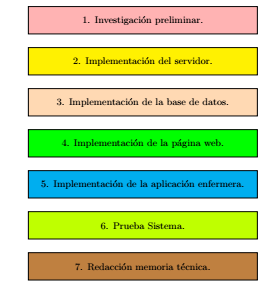
\includegraphics[width=.7\textwidth]{./Figuras/AoN-2.png}
\caption{Colores del diagrama de \textit{Activity on Node}.}
\label{fig:AoN0}

\end{figure}


En la figura 3 se presenta el diagrama de \textit{Activity on Node}, donde el camino crítico es indicado mediante una linea de interconexión resaltada:
\begin{figure}[htpb]
\centering 
\includegraphics[width=1\textwidth]{./Figuras/diagramaAoN.png}
\caption{Diagrama de \textit{Activity on Node}.}
\label{fig:AoN}
\end{figure}


\section{11. Diagrama de Gantt}
\label{sec:gantt}
En la siguiente figura se presenta la lista de tareas ingresadas al sistema de gestión de tareas y el diagrama de Gantt con las tareas acordes con el diagrama de \textit{Activity on Node}.

\begin{landscape}
\begin{figure}

\centering 
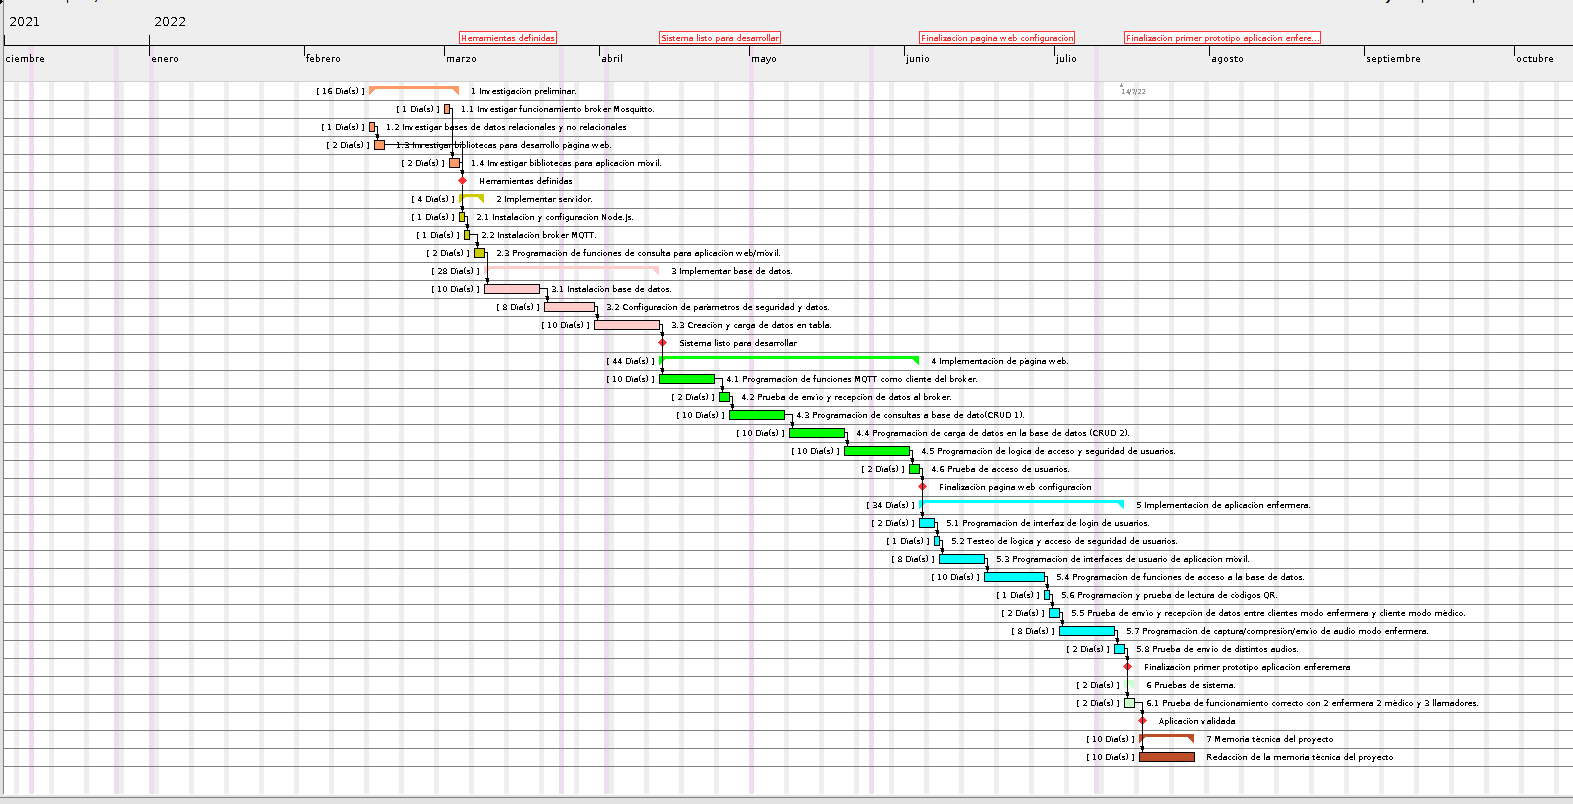
\includegraphics[height=.85\textheight]{./Figuras/tareas.png}
\caption{Planificación de tareas.}
\label{fig:diagGantt0}

\end{figure}
\end{landscape}
%\begin{consigna}{red}

%Pegar acá una captura de pantalla del diagrama de Gantt, cuidando que la letra sea suficientemente grande como para ser legible. 
%Si el diagrama queda demasiado ancho, se puede pegar primero la ``tabla'' del Gantt y luego pegar la parte del diagrama de barras del diagrama de Gantt.

%Configurar el software para que en la parte de la tabla muestre los códigos del EDT (WBS).\\
%Configurar el software para que al lado de cada barra muestre el nombre de cada tarea.\\
%Revisar que la fecha de finalización coincida con lo indicado en el Acta Constitutiva.

%En la figura \ref{fig:gantt}, se muestra  un ejemplo de diagrama de gantt realizado con el paquete de \textit{pgfgantt}. En la plantilla pueden ver %el código que lo genera y usarlo de base para construir el propio.

%\begin{figure}[htbp]
%\begin{center}
%\begin{ganttchart}{1}{12}
%  \gantttitle{2020}{12} \\
%  \gantttitlelist{1,...,12}{1} \\
%  \ganttgroup{Group 1}{1}{7} \\
%  \ganttbar{Task 1}{1}{2} \\
%  \ganttlinkedbar{Task 2}{3}{7} \ganttnewline
%  \ganttmilestone{Milestone o hito}{9} \ganttnewline
%  \ganttbar{Final Task}{8}{12}
%  \ganttlink{elem2}{elem3}
%  \ganttlink{elem3}{elem4}
%\end{ganttchart}
%\end{center}
%\caption{Diagrama de gantt de ejemplo}
%\label{fig:gantt}
%\end{figure}


%\begin{figure}[htbp]
%\begin{center}
%\begin{ganttchart}{1}{12}
%  \gantttitle{2020}{12} \\
%  \gantttitlelist{1,...,12}{1} \\
%  \ganttgroup{Group 1}{1}{7} \\
%  \ganttbar{Task 1}{1}{2} \\
%  \ganttlinkedbar{Task 2}{3}{7} \ganttnewline
%  \ganttmilestone{Milestone o hito}{7} \ganttnewline
%  \ganttbar{Final Task}{8}{12}
%  \ganttlink{elem2}{elem3}
%  \ganttlink{elem3}{elem4}
%\end{ganttchart}
%\end{center}
%\caption{Diagrama de gantt de ejemplo}
%\label{fig:gantt}
%\end{figure}



\begin{landscape}
\begin{figure}[htpb]
\centering 
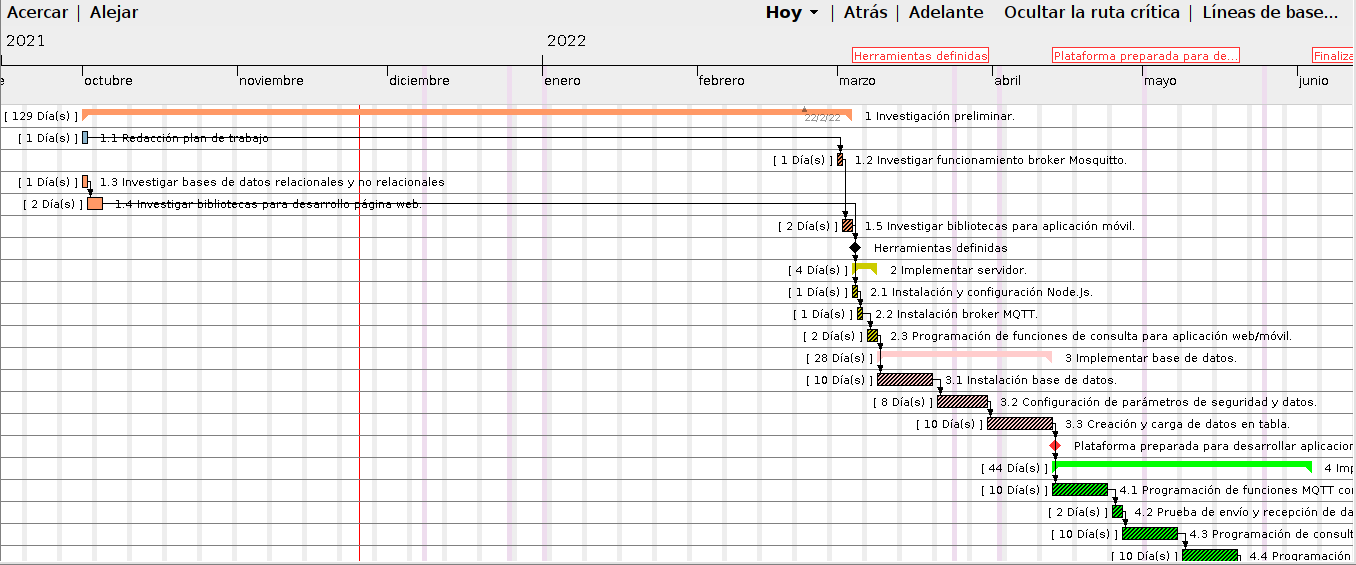
\includegraphics[height=.60\textheight]{./Figuras/planning1.png}
\caption{Diagrama de Gantt (continua en la página siguiente).}
\label{fig:diagGantt}
\end{figure}
\end{landscape}


\newpage
\begin{landscape}
\begin{figure}[htpb]
\centering 
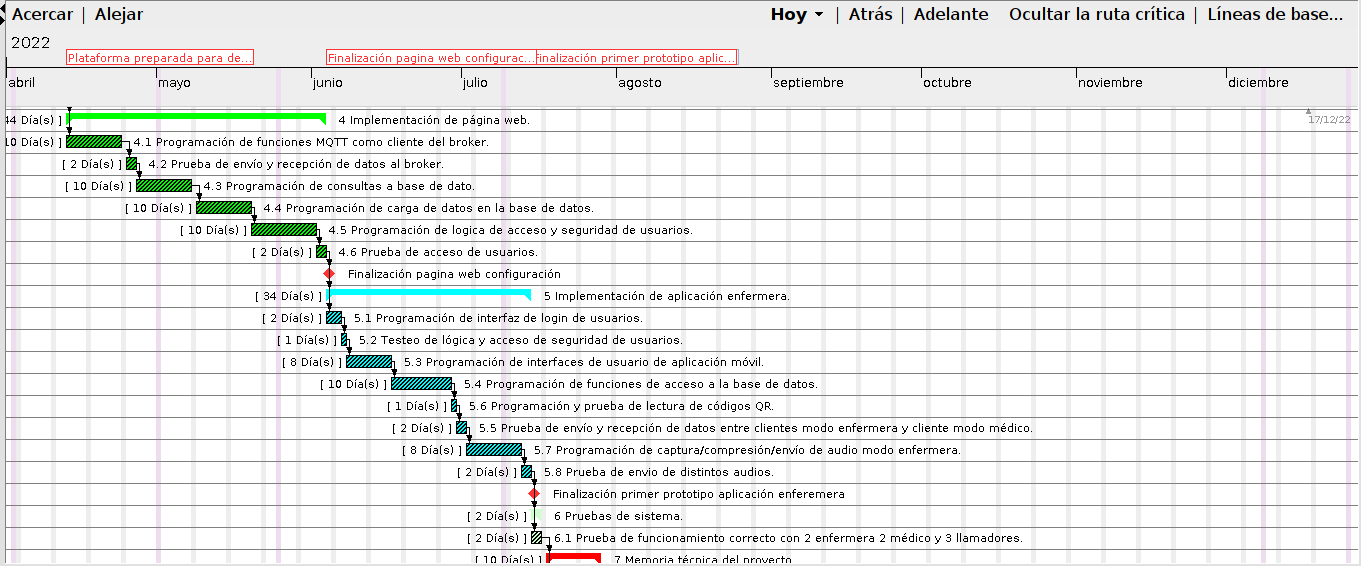
\includegraphics[height=.60\textheight]{./Figuras/planning2.png}
\caption{Diagrama de Gantt (continua en la página siguiente).}
\label{fig:diagGantt2}
\end{figure}
\end{landscape}

\newpage
\begin{landscape}
\begin{figure}[htpb]
\centering 
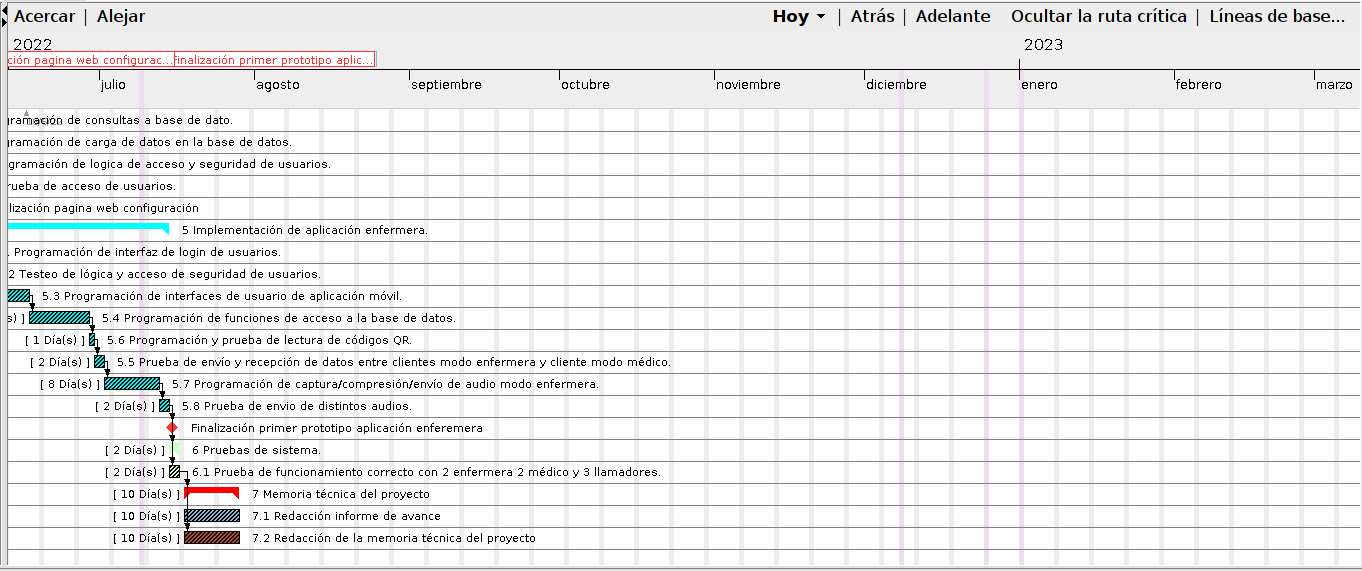
\includegraphics[height=.60\textheight]{./Figuras/planning3.png}
\caption{Diagrama de Gantt.}
\label{fig:diagGantt3}
\end{figure}

\end{landscape}

\section{12. Presupuesto detallado del proyecto}
\label{sec:presupuesto}

%\begin{consigna}{red}
%Si el proyecto es complejo entonces separarlo en partes:
%\begin{itemize}
%	\item Un total global, indicando el subtotal acumulado por cada una de las áreas.
%	\item El desglose detallado del subtotal de cada una de las áreas.
%\end{itemize}

%IMPORTANTE: No olvidarse de considerar los COSTOS INDIRECTOS.

%\end{consigna}

En la siguiente tabla se presentan los gastos previstos del proyecto, expresados en pesos argentinos.

\begin{table}[htpb]
\centering
\begin{tabularx}{\linewidth}{@{}|X|c|r|r|@{}}
\hline
\rowcolor[HTML]{C0C0C0} 
\hline
\multicolumn{4}{|c|}{\cellcolor[HTML]{C0C0C0}COSTOS DIRECTOS} \\ \hline
\rowcolor[HTML]{C0C0C0} 
Descripción &
  \multicolumn{1}{|l|}{\cellcolor[HTML]{C0C0C0}Cantidad} &
  \multicolumn{1}{|l|}{\cellcolor[HTML]{C0C0C0}Valor unitario(\$)} &
  \multicolumn{1}{|l|}{\cellcolor[HTML]{C0C0C0}Valor total(\$)} \\ \hline
 Investigación &
  \multicolumn{1}{|l|}{70hs}&
  \multicolumn{1}{|l|}{1000}&
  \multicolumn{1}{|l|}{70000} \\ \hline
 Programación&
  \multicolumn{1}{|l|}{424hs} &
  \multicolumn{1}{|l|}{1000} &
  \multicolumn{1}{|l|}{424000} \\ \hline
 Testing&
  \multicolumn{1}{|l|}{66hs} &
  \multicolumn{1}{|l|}{1000} &
  \multicolumn{1}{|l|}{66000} \\ \hline 
 Documentación&
  \multicolumn{1}{|l|}{60hs} &
  \multicolumn{1}{|l|}{1000} &
  \multicolumn{1}{|l|}{60000} \\ \hline  

\multicolumn{3}{|c|}{SUBTOTAL} &
  \multicolumn{1}{|l|}{620000} \\ \hline

\rowcolor[HTML]{C0C0C0} 
\hline
\multicolumn{4}{|c|}{\cellcolor[HTML]{C0C0C0}COSTOS INDIRECTOS} \\ \hline
\rowcolor[HTML]{C0C0C0} 
Descripción &
  \multicolumn{1}{c|}{\cellcolor[HTML]{C0C0C0}Cantidad} &
  \multicolumn{1}{c|}{\cellcolor[HTML]{C0C0C0}Valor unitario(\$)} &
  \multicolumn{1}{c|}{\cellcolor[HTML]{C0C0C0}Valor total(\$)} \\ \hline
\multicolumn{1}{|l|}{Raspberry pi 4(Server)} &
  \multicolumn{1}{|l|}{1} &
  \multicolumn{1}{|l|}{27000} &
   \multicolumn{1}{|l|}{27000} 
   \\ \hline
\multicolumn{1}{|l|}{Costos de Consumo eléctrico} &
  \multicolumn{1}{|l|}{600} &
  \multicolumn{1}{|l|}{4} &
  \multicolumn{1}{|l|}{2400} 
   \\ \hline
%\multicolumn{1}{|l|}{Asesorías} &
%  \multicolumn{1}{|l|}{20hs} &
%  \multicolumn{1}{|l|}{1000} &
%  \multicolumn{1}{|l|}{20000} 
%   \\ \hline
\multicolumn{3}{|c|}{SUBTOTAL} &
  \multicolumn{1}{|l|}{29400} \\ \hline
\rowcolor[HTML]{C0C0C0}
\multicolumn{3}{|l|}{TOTAL} &
\multicolumn{1}{|l|}{649400} \\ \hline

\end{tabularx}%
\end{table}


\section{13. Gestión de riesgos}
\label{sec:riesgos}

Para clasificación de los riesgos se utiliza dos características: 
\begin{itemize}
\item Severidad del evento o la situación: indica cuanto afecta a la ejecución del proyecto en tiempo y forma. Se lo clasifica con un indice numérico y los límites de la escala son:  1 no afecta al proyecto y 10  imposibilita la ejecución del mismo.
\item Ocurrencia: indica cuan probable es que el evento o la situación ocurra. Se clasifica de 1 a 10, siendo 1 muy poco probable y 10 muy probable. 
\end{itemize}

En este proyecto se detectaron los siguientes riesgos:

 
Riesgo 1: no contar con un dispositivo de los necesarios para el testeo de las aplicaciones.
\begin{itemize}
	\item Severidad (S): 10.\newline 
	Justificación: al ser la aplicación multiplataforma, es menester contar con un dispositivo Android, un dispositivo IOS y una pc con navegador web.
	\item Probabilidad de ocurrencia (O): 5.\newline 
	Justificación: en este momento no se posee un dispositivo IOS pero existen posibilidades de acceder a uno.
\end{itemize}   

Riesgo 2: disminución de tiempo disponible para la realización del plan trazado.
\begin{itemize}
	\item Severidad (S): 7. \newline 
	Justificación: el disminuir el tiempo diario asignado a cada tarea, retrasa todo el calendario.
	\item Ocurrencia (O):3. \newline 
	Justificación: la planificación es correcta y es muy poco probable que surjan actividades adicionales que ocupen al recurso humano.
\end{itemize}

Riesgo 3: daño en equipamiento utilizado en el proyecto por problemas en el suministro eléctrico.
\begin{itemize}
	\item Severidad (S): 10.\newline 
	Justificación: genera retrasos temporales y modificaciones al presupuesto ya que se deben adquirir nuevos recursos materiales, instalar el framework de desarrollo y acondicionarlo para continuar el proyecto.
	\item Ocurrencia (O): 3.\newline 
	Justificación: en estos momentos el equipamiento se encuentra protegido mediante un estabilizador de tensión.
\end{itemize}	
Riesgo 4: no contar con colaboradores para realizar la validación del sistema.
\begin{itemize}
	\item Severidad (S): 5.\newline 
	Justificación: es necesario que los colaboradores sean idóeos.
	\item Ocurrencia (O): 8.\newline 
	Justificación: debido a que los colaboradores poseen otras tareas en su trabajo puede que no dispongan del tiempo necesario a las pruebas.
\end{itemize}
Riesgo 5: surgimiento de una alternativa con mejores prestaciones a la sugerida en el plan de trabajo (nueva librería, framework, etc).
\begin{itemize}
	\item Severidad (S): 1.\newline 
	Justificación: el surgimiento de una nueva alternativa con mejores prestaciones a la elegida para el desarrollo puede dejar al producto en una posición de desventaja respecto a la competencia. No obstante, el utilizar tecnologías ya probadas asegura un nivel de confianza mayor en cuanto a seguridad y estabilidad a lo largo del tiempo.
	\item Ocurrencia (O): 10.\newline 
	Justificación: en el rubro informático continuamente surgen nuevas alternativas para el desarrollo. 	
		 
	
\end{itemize}

\newpage
b) Tabla de gestión de riesgos:      (El RPN se calcula como RPN=SxO)

\begin{table}[htpb]
\centering
\begin{tabularx}{\linewidth}{@{}|X|c|c|c|c|c|c|@{}}
\hline
\rowcolor[HTML]{C0C0C0} 
Riesgo & S & O & RPN & S* & O* & RPN* \\ \hline
1.No contar con un dispositivo de los necesario para el testeo de las aplicaciones.    &   10 & 5  &  50  &  5  & 1   & 5   \\ \hline
2.Disminución de tiempo disponible para la realización del plan trazado       & 7  & 3  & 21    &    &    &      \\ \hline
3.Daño en equipamiento utilizado en el proyecto por problemas en el suministro eléctrico       & 10  & 3  & 30    &  1  &   1 &     1 \\ \hline
4.No contar con colaboradores para realizar la validación del sistema.     & 5  & 8 & 40    &  5  &  2  &    10  \\ \hline
5.Surgimiento de una alternativa con mejores prestaciones a la sugerida en el plan de trabajo       & 1  & 10 & 10    &    &    &      \\ \hline
\end{tabularx}%
\end{table}

Criterio adoptado: 
Se tomarán medidas de mitigación en los riesgos cuyos números de RPN sean mayores a 25.

Nota: los valores marcados con (*) en la tabla corresponden luego de haber aplicado la mitigación.

c) Plan de mitigación de los riesgos que originalmente excedían el RPN máximo establecido:

%Riesgo 1: plan de mitigación (si por el RPN fuera necesario elaborar un plan de mitigación).
 % Nueva asignación de S y O, con su respectiva justificación:
 % - Severidad (S): mientras más severo, más alto es el número (usar números del 1 al 10).
  %        Justificar el motivo por el cual se asigna determinado número de severidad (S).
  %- Probabilidad de ocurrencia (O): mientras más probable, más alto es el número (usar del 1 al 10).
  %        Justificar el motivo por el cual se asigna determinado número de (O).
          
Riesgo 1: se buscarán contactos conocidos que posean un dispositivo de esas características.
-Severidad(S) : 5.\newline
	Justificación: impide la validación del sistema en una plataforma.\newline
-Ocurrencia: 1.\newline
	Justificación: es muy improbable que al momento de la validación no se encuentre el recurso.


Riesgo 3: se incorporará un sistema de alimentación ininterrumpible (UPS,  Uninterruptable Power Supply) y se mantendrá todo progreso del trabajo en servidores en la nube.\newline
-Severidad(S) : 1.\newline
Justificación: al tener un equipo de backup y todo lo trabajado en la nube, no existe posibilidad de demoras por este motivo.\newline
-Ocurrencia: 1.\newline
Justificación: al incorporar la UPS, los daños a los discos rígidos se anulan.
 
Riesgo 4: se gestiona una lista de contactos que se encargarán de validar el sistema y se genera un compromiso con los mismos.\newline
-Severidad(S) : 5.\newline
Justificación: no se modifica la severidad del mismo.
\newline
-Ocurrencia: 2.\newline
Justificación: al haber varios contactos, la imposibilidad simultánea de todos es improbable.\newline

\section{14. Gestión de la calidad}
\label{sec:calidad}

\begin{itemize}

\item Req 1: requisitos de el servidor(agrupo los subrequisitos 1.1,1.2 y 1.3).
	\begin{itemize}
	\item Verificación: se verificará que el servidor MOSQUITTO MQTT se encuentre en condiciones de ser utilizado y acepte comunicación con aplicaciones standares de clientes MQTT.
	\item Validación: no aplica.
	\end{itemize}


\item Req 2: requerimientos relativos a la base de datos(agrupo 2.1,2.2 y 2.3).
	\begin{itemize}
	\item Verificación: se verificará la presencia de la base de dato, con las tablas definidas y el correcto funcionamiento de los endpoints con programas de prueba.
	\item Validación: no aplica.
	\end{itemize}


\item Req 3.1 y 3.2: La página web debe poder consultar y modificar a la base de datos.
	\begin{itemize}
	\item Verificación: se verificará que desde la página se puedan cargar/editar/consultar datos de la base de datos.
	\item Validación:  no aplica.
	\end{itemize}
\item Req 3.3: La página web debe permitir obtener estadísticas de pacientes o enfermeras.
	\begin{itemize}
	\item Verificación: se verificará que desde la página se pueda consultar cuantas veces por día se atiende a un paciente y cuantos pacientes atendió una enfermera.
	\item Validación:  no aplica.
	\end{itemize}	
\item Req 3.4: La página web contener acceso con usuario y contraseña para cada persona.
	\begin{itemize}
	\item Verificación: se verificará el funcionamiento según el usuario logeado.
	\item Validación:  no aplica.
	\end{itemize}		
	

\item Req 4.1 y 4.2 La aplicación móvil debe tener 3 modos de uso: usuario médico, usuario enfermera y usuario sistema. El modo de uso se activa luego de logearse el usuario.
	\begin{itemize}
	\item Verificación: se verificará el funcionamiento logeandose de distintos modos.
	\item Validación: no aplica.
	\end{itemize}		
	
\item Req 4.3 y 4.4 La aplicación en modo enfermera debe poder descargar información del paciente y debe permitir leer código QR.
	\begin{itemize}
	\item Verificación: se verificará el funcionamiento utilizando un código QR específico que identifique la cama en la base de datos y se verificará que pueda descargar información del paciente.
	\item Validación: no aplica.
	\end{itemize}		


\item Req 4.5: La aplicación en modo sistema debe mostrar las habitaciones sin atención, según una tabla de prioridades y en caso de igualdad de prioridades, mostrar según el orden de llamada.
	\begin{itemize}
	\item Verificación: se carga una tabla de prioridades por habitacióny se verifica el funcionamiento cuando se realizan simulaciones de distintas situaciones.
	\item Validación:  No aplica.
	\end{itemize}	

\item Req 4.6: El modo usuario médico y el modo usuario enfermera deben poder enviar mensajes de textos o sonido comprimido en 32kbps(mp3)
	\begin{itemize}
	\item Verificación: se realiza una simulación enviando un audio de enfermera a médico y de médico a enfermera.
	\item Validación:  se valida con ayuda de los colaboradores en un entorno real junto con todo el sistema.
	\end{itemize}		

\item Req 5: requisitos de documentación(agrupados 5.1 y 5.2).

	\begin{itemize}
	\item Verificación: se verifica la presencia de la documentación de cada software.
	\item Validación: no aplica.
	\end{itemize}	
		
\item Req 6: requisitos del sistema completo.

	\begin{itemize}
	\item Verificación: se realiza una simulación de funcionamiento del sistema en el laboratorio.
	\item Validación: Se entregará el prototipo de todo el sistema y las aplicaciones a los colaboradores para que lo utilicen durante una semana y se evaluará los resultados.
	\end{itemize}		

\item Req 7: requisitos de entregas.

	\begin{itemize}
	\item Verificación: se comprueba la presencia de los contenedores con el código fuente generado. Se descargan y se regenera todo el sistema nuevamente.
	\item Validación: no aplica.
	\end{itemize}			

\end{itemize}

\section{15. Procesos de cierre}    
\label{sec:cierre}

%\begin{consigna}{red}
%Establecer las pautas de trabajo para realizar una reunión final de evaluación del proyecto, tal que contemple las siguientes actividades:

%\begin{itemize}
%	\item Pautas de trabajo que se seguirán para analizar si se respetó el Plan de Proyecto original:
%	 - Indicar quién se ocupará de hacer esto y cuál será el procedimiento a aplicar. 
%	\item Identificación de las técnicas y procedimientos útiles e inútiles que se emplearon, y los problemas que surgieron y cómo se solucionaron:
%	 - Indicar quién se ocupará de hacer esto y cuál será el procedimiento para dejar registro.
%	\item Indicar quién organizará el acto de agradecimiento a todos los interesados, y en especial al equipo de trabajo y colaboradores:
%	  - Indicar esto y quién financiará los gastos correspondientes.
%\end{itemize}

%\end{consigna}
Al finalizar el proyecto se realizará una evaluación final que contemple las siguientes actividades:
\begin{itemize}


\item El responsable del proyecto analizará el cumplimiento del plan del proyecto con sus tiempos indicados y se evaluará los requerimientos no cumplidos.
\item Se evaluarán los riesgos previstos que efectivamente se hayan manifestado, y el procedimiento de mitigación planificado versus el real. Se evaluaran demoras causadas por eventos no previstos.
\item El responsable del proyecto realiza una presentación pública del resultado del proyecto asi como del historial de su desarollo.
\end{itemize}

\end{document}
